\RequirePackage{atbegshi}
\documentclass[compress,dvipsnames, aspectratio=169]{beamer} % aspectratio=169
%\usepackage[svgnames]{xcolor}

%	%	%	%	%	%	%	%	%	%	%	%	%	%	%
% 						MY PACKAGES 
%	%	%	%	%	%	%	%	%	%	%	%	%	%	%
\usepackage{graphicx}				% Use pdf, png, jpg, or eps with pdflatex; use eps in DVI mode

\usepackage[export]{adjustbox}

\usepackage{amssymb}
\usepackage{amsmath}	
%\usepackage{tipx}
%\usepackage{tikz}
%\usetikzlibrary{arrows,shapes,decorations.pathmorphing,backgrounds,positioning,fit,petri}
\usepackage{rotating}
\usepackage{scalerel} % for inline images
\usepackage{import}
%\usepackage{times}
\usepackage{array}
\usepackage{tabularx}
%\usepackage{booktabs}
\usepackage{textcomp}
\usepackage{caption}
\usepackage{booktabs}
\usepackage{float}
\usepackage{pbox}
%\usepackage{setspace} 			% \doublespacing \singlespacing \onehalfspacing	%doble espacio
%\label{x:y}													%ocupar para autoref.
%\autoref{x:y}												%ocupar para autoref.
%\usepackage{nopageno}			%desactivar para p�ginas
\usepackage{pifont}
\usepackage{color,xcolor,ucs}
%\usepackage{marvosym} %faces

\usepackage{hyperref}
\usepackage{multirow}

\usepackage{listings}
\usepackage{color}
\definecolor{dkgreen}{rgb}{0,0.6,0}
\definecolor{gray}{rgb}{0.5,0.5,0.5}
\definecolor{mauve}{rgb}{0.58,0,0.82}
\lstset{ %
  language=R,                     % the language of the code
  basicstyle=\TINY,      			% the size of the fonts that are used for the code
  numbers=left,                   % where to put the line-numbers
  numberstyle=\tiny\color{gray},  % the style that is used for the line-numbers
  stepnumber=1,                   % the step between two line-numbers. If it's 1, each line
                                  % will be numbered
  numbersep=5pt,                  % how far the line-numbers are from the code
  backgroundcolor=\color{white},  % choose the background color. You must add \usepackage{color}
  showspaces=false,               % show spaces adding particular underscores
  showstringspaces=false,         % underline spaces within strings
  showtabs=false,                 % show tabs within strings adding particular underscores
  frame=single,                   % adds a frame around the code
  rulecolor=\color{black},        % if not set, the frame-color may be changed on line-breaks within not-black text (e.g. commens (green here))
  tabsize=1,                      % sets default tabsize to 2 spaces
  captionpos=b,                   % sets the caption-position to bottom
  breaklines=true,                % sets automatic line breaking
  breakatwhitespace=false,        % sets if automatic breaks should only happen at whitespace
  title=\lstname,                 % show the filename of files included with \lstinputlisting;
                                  % also try caption instead of title
  keywordstyle=\color{blue},      % keyword style
  commentstyle=\color{dkgreen},   % comment style
  stringstyle=\color{mauve},      % string literal style
  escapeinside={\%*}{*)},         % if you want to add a comment within your code
  morekeywords={*,...}            % if you want to add more keywords to the set
} 

%	%	%	%	%	%	%	%	%	%	%	%	%	%	%
% 					PACKAGE CUSTOMIZATION
%	%	%	%	%	%	%	%	%	%	%	%	%	%	%

% GENERAL CUSTOMIZATION
\usepackage[math]{iwona}% font
\usetheme{Singapore}	% template I should use
%\usetheme{Szeged}	% alternative template
\usecolortheme{rose}	% color template
\makeatletter			% to show subsection/section title (1/3)
\beamer@theme@subsectiontrue % to show subsection/section title (2/3)
\makeatother			% to show subsection/section title (3/3)


% THIS BELOW IS TO MAKE NAVIGATION DOTS MARKED DURING PRESENTATION
\makeatletter
\def\slideentry#1#2#3#4#5#6{%
  %section number, subsection number, slide number, first/last frame, page number, part number
  \ifnum#6=\c@part\ifnum#2>0\ifnum#3>0%
    \ifbeamer@compress%
      \advance\beamer@xpos by1\relax%
    \else%
      \beamer@xpos=#3\relax%
      \beamer@ypos=#2\relax%
    \fi%
  \hbox to 0pt{%
    \beamer@tempdim=-\beamer@vboxoffset%
    \advance\beamer@tempdim by-\beamer@boxsize%
    \multiply\beamer@tempdim by\beamer@ypos%
    \advance\beamer@tempdim by -.05cm%
    \raise\beamer@tempdim\hbox{%
      \beamer@tempdim=\beamer@boxsize%
      \multiply\beamer@tempdim by\beamer@xpos%
      \advance\beamer@tempdim by -\beamer@boxsize%
      \advance\beamer@tempdim by 1pt%
      \kern\beamer@tempdim
      \global\beamer@section@min@dim\beamer@tempdim
      \hbox{\beamer@link(#4){%
          \usebeamerfont{mini frame}%
          \ifnum\c@section>#1%
            %\usebeamercolor[fg]{mini frame}%
            %\usebeamertemplate{mini frame}%
            \usebeamercolor{mini frame}%
            \usebeamertemplate{mini frame in other subsection}%
          \else%
            \ifnum\c@section=#1%
              \ifnum\c@subsection>#2%
                \usebeamercolor[fg]{mini frame}%
                \usebeamertemplate{mini frame}%
              \else%
                \ifnum\c@subsection=#2%
                  \usebeamercolor[fg]{mini frame}%
                  \ifnum\c@subsectionslide<#3%
                    \usebeamertemplate{mini frame in current subsection}%
                  \else%
                    \usebeamertemplate{mini frame}%
                  \fi%
                \else%
                  \usebeamercolor{mini frame}%
                  \usebeamertemplate{mini frame in other subsection}%
                \fi%
              \fi%
            \else%
              \usebeamercolor{mini frame}%
              \usebeamertemplate{mini frame in other subsection}%
            \fi%
          \fi%
        }}}\hskip-10cm plus 1fil%
  }\fi\fi%
  \else%
  \fakeslideentry{#1}{#2}{#3}{#4}{#5}{#6}%
  \fi\ignorespaces
  }
\makeatother

%	%	%	%	%	%	%	%	%	%	%	%	%	%	%
% 			To show the TITLE at the Bottom of each slide
%	%	%	%	%	%	%	%	%	%	%	%	%	%	%

\beamertemplatenavigationsymbolsempty 
\makeatletter
\setbeamertemplate{footline}
{
\leavevmode%
\hbox{%
\begin{beamercolorbox}[wd=1\paperwidth,ht=2.25ex,dp=2ex,center]{title in head/foot}%
\usebeamerfont{title in head/foot}\insertshorttitle
\end{beamercolorbox}%
\begin{beamercolorbox}[wd=1
\paperwidth,ht=2.25ex,dp=2ex,center]{date in head/foot}%
\end{beamercolorbox}}%
}
\makeatother


\lstdefinestyle{base}{
  language=tex,
  emptylines=1,
  breaklines=true,
  basicstyle=\tiny\color{black},
  moredelim=**[is][\color{red}]{@}{@},
  frame=lrtb,
  numbers=none
}





% to switch off navigation bullets
%% using \miniframeson or \miniframesoff
\makeatletter
\let\beamer@writeslidentry@miniframeson=\beamer@writeslidentry
\def\beamer@writeslidentry@miniframesoff{%
  \expandafter\beamer@ifempty\expandafter{\beamer@framestartpage}{}% does not happen normally
  {%else
    % removed \addtocontents commands
    \clearpage\beamer@notesactions%
  }
}
\newcommand*{\miniframeson}{\let\beamer@writeslidentry=\beamer@writeslidentry@miniframeson}
\newcommand*{\miniframesoff}{\let\beamer@writeslidentry=\beamer@writeslidentry@miniframesoff}
\makeatother

% Image full size: use 
%%\begin{frame}
  %%\fullsizegraphic{monogram.jpg}
%%\end{frame}
\newcommand<>{\fullsizegraphic}[1]{
  \begin{textblock*}{0cm}(-1cm,-3.78cm)
  \includegraphics[width=\paperwidth]{#1}
  \end{textblock*}
}


% hyperlinks
\hypersetup{colorlinks,
            urlcolor=[rgb]{0.01, 0.28, 1.0},
            linkcolor=[rgb]{0.01, 0.28, 1.0}}








%	%	%	%	%	%	%	%	%	%	%	%	%	%	%
% 					DOCUMENT ID
%	%	%	%	%	%	%	%	%	%	%	%	%	%	%

\title{Interview with Turku University}
\author{Hector Bahamonde $\bullet$ Assistant Professor $\bullet$ O'Higgins University (Chile)}
\date{June 22nd, 2021}

%to to see shadows of previous blocks
%\setbeamercovered{dynamic}


\begin{document}



%	%	%	%	%	%	%	%	%	%	%	%	%	%	%
% 					CONTENT
%	%	%	%	%	%	%	%	%	%	%	%	%	%	%

%% title frame

\begin{frame}[label = beginning]
\titlepage
\end{frame}



\section{Introduction}

%section{Outline}
\subsection{Introduction}

\miniframesoff
\begin{frame}\frametitle{The Order of the Day}
In this presentation I will...
\begin{enumerate}
	\item Briefly describe my {\bf profile}.
	\item Quickly mention three of my most important {\bf publications}.
	\item Explain my 3-year {\bf research plan} at Turku.
	\item Enumerate the three main reasons to {\bf move to Turku}.
\end{enumerate}
\end{frame}


\subsection{Short Bio}

\miniframeson
\begin{frame}\frametitle{Short Bio}
I am a political scientist (B.A. and PhD).
\begin{itemize}
	\item Study the political economy of {\bf inequality}, {\bf democracy} and {\bf clientelism}. 
	\item Make heavy use of statistical and experimental methods (natural, lab and survey-based).
	\item Currently an assistant professor in Chile---but looking forward to relocate to Europe; family reasons. {\bf Immediate availability}.
\end{itemize}
\end{frame}

\subsection{Published Work}


%\miniframeson
%\begin{frame}\frametitle{Main Published Work}
%	\begin{enumerate}
%		\item ``{\bf Inclusive Institutions, Unequal Outcomes: Democracy, State Capacity, and Income Inequality}.''
%			\begin{itemize}
%				\item {\color{ForestGreen}Democratic theory, inequality and stateness}.
%				\item Time-series and fixed-effects methods.
%				\item {\color{blue}European Journal of Political Economy} (forthcoming).
%			\end{itemize}
%		\item ``{\bf Still for Sale: The Micro-Dynamics of Vote Selling in the United States, Evidence From a List Experiment}.''
%			\begin{itemize}
%				\item {\color{ForestGreen}Democratic development and clientelism}.
%				\item Survey experiment (list experiment) implemented via \texttt{Qualtrics}.
%				\item \emph{Original} data representative at the U.S. level.
%				\item {\color{blue}Acta Politica} (forthcoming).
%			\end{itemize}
%		\item ``{\bf Aiming Right at You: Group versus Individual Clientelistic Targeting in Brazil}.''
%			\begin{itemize}
%				\item {\color{ForestGreen}Inequality and clientelism}. 
%				\item Observational data and matching methods for causal inference.
%				\item {\color{blue}Journal of Politics in Latin America} (2018).
%			\end{itemize}
%	\end{enumerate}
%\end{frame}


\miniframeson
\begin{frame}\frametitle{``{\bf Inclusive Institutions, Unequal Outcomes: Democracy, State Capacity, and Income Inequality}.''}
	\begin{columns}
	\column{0.5\textwidth}
			\begin{itemize}
				\item {\color{ForestGreen}Global democratic theory, inequality and stateness}.
				\item 126 industrial and developing countries, between 1970 and 2013 (N=4,000).
				\item Time-series and fixed-effects methods.
				\item {\tiny European Journal of Political Economy (forthcoming).}
			\end{itemize}

	\column{0.5\textwidth}
		\begin{figure}[H]
		%\vspace{-2.5cm}
		\hspace{-7mm}
		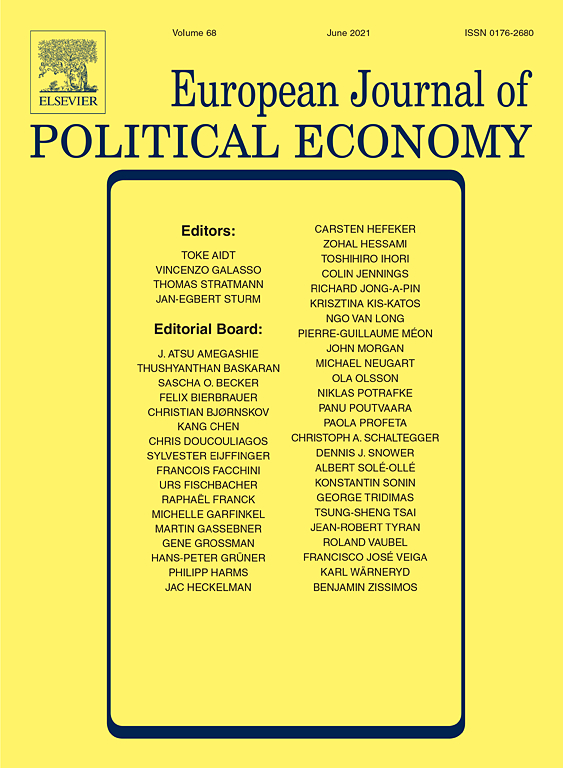
\includegraphics[scale=0.2]{/Users/hectorbahamonde/Job_Market/cover_ejpe.jpg}
		\end{figure}
	
	\end{columns}

\vspace{\fill}\hspace{\fill}\hyperlink{mart_paper}{\beamerbutton{Details}}

\end{frame}


\miniframesoff
\begin{frame}\frametitle{``{\bf Still for Sale: The Micro-Dynamics of Vote Selling in the United States, Evidence From a List Experiment}.''}
	\begin{columns}
	\column{0.5\textwidth}
			\begin{itemize}
				\item {\color{ForestGreen}Democratic development and clientelism in the United States}.
				\item I designed a survey experiment (list experiment) and implemented it in \texttt{Qualtrics}.
				\item \emph{Original} data representative at the U.S. level.
				\item {\tiny Acta Politica (forthcoming).}
			\end{itemize}

	\column{0.5\textwidth}
		\begin{figure}[H]
		%\vspace{-2.5cm}
		\hspace{-7mm}
		
\includegraphics[scale=0.3]{/Users/hectorbahamonde/Job_Market/cover_ap.jpeg}
		\end{figure}
	\end{columns}

\vspace{\fill}\hspace{\fill}\hyperlink{vote_selling_paper}{\beamerbutton{Details}}

\end{frame}


\miniframesoff
\begin{frame}\frametitle{``{\bf Aiming Right at You: Group versus Individual Clientelistic Targeting in Brazil}.''}
	\begin{columns}
	\column{0.5\textwidth}
			\begin{itemize}
				\item {\color{ForestGreen}Inequality and clientelism in Brazil}. 
				\item Observational data and matching methods for causal inference.
				\item {\tiny Journal of Politics in Latin America (2018).}
			\end{itemize}

	\column{0.5\textwidth}
		\begin{figure}[H]
		%\vspace{-2.5cm}
		\hspace{-7mm}
		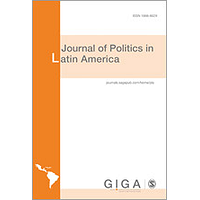
\includegraphics[scale=0.2]{/Users/hectorbahamonde/Job_Market/cover_jpla.png}
		\end{figure}
	\end{columns}

\vspace{\fill}\hspace{\fill}\hyperlink{brazil_paper}{\beamerbutton{Details}}

\end{frame}





\section{Research Plan}

\subsection{Pipeline summary}

\miniframesoff
\begin{frame}
\centering
\huge{My research plan seeks to study these issues by moving forward several pieces of research I have in the pipeline.}
\end{frame}

% HERE


\miniframeson
\begin{frame}\frametitle{Research Plan: Two Pipelines}
\begin{enumerate} \setcounter{enumi}{0}
\item {\color{ForestGreen}Clientelism and Democratic Theory}: {\bf lab and survey experiments}.
	\begin{itemize}
		\item \scriptsize{``{\input{/Users/hectorbahamonde/research/Economic_Experiment_Vote_Selling/title.txt}\unskip}'' ({\color{blue}{\input{/Users/hectorbahamonde/research/Economic_Experiment_Vote_Selling/status.txt}\unskip}}).}
		
		\item \scriptsize{``{\input{/Users/hectorbahamonde/research/Conjoint_US/title_letter.txt}\unskip}'' ({\color{blue}{\input{/Users/hectorbahamonde/research/Conjoint_US/status_letter.txt}\unskip}}).}

	\end{itemize}

		\item {\color{ForestGreen}Inequality and Covid}: {\bf natural experiments}.

	\begin{itemize}
		\item \scriptsize{``{\input{/Users/hectorbahamonde/research/Tobalaba/title.txt}\unskip}'' ({\color{blue}{\input{/Users/hectorbahamonde/research/Tobalaba/status.txt}\unskip}}).}
		
		\item \scriptsize{``{\input{/Users/hectorbahamonde/research/Bus/title.txt}\unskip}'' ({\color{blue}{\input{/Users/hectorbahamonde/research/Bus/status.txt}\unskip}}).}
	\end{itemize}


\end{enumerate}
\end{frame}



\subsection{Pipeline 1: survey and lab experiments}

\miniframeson
\begin{frame}\frametitle{{\scriptsize{``\input{/Users/hectorbahamonde/research/Economic_Experiment_Vote_Selling/title.txt}\unskip.}''}}
	%\begin{columns}
	%\column{0.5\textwidth}
		\begin{itemize}
			\item {\color{blue}Economic experiment (``game'')}: subjects represent randomly-assigned roles {\scriptsize(2 parties/1 voter)}.
		\end{itemize}
		
		\begin{enumerate}	
			\item {\color{ForestGreen}Behavioral economics framework}, play a game of {\color{blue}deliberation}: subjects make decisions and get payed according to the quality of their decisions.

			\item {\color{ForestGreen}Democratic theory}: study conditions of {\bf (i)lliberal democracy} that foster clientelism. Randomize different:
						\begin{itemize}
							\item {\bf Endowments}: ``parties'' and ``voters'' {\scriptsize({\color{blue}emulates income inequality})}.
							\item {\bf Ideology}: ``parties'' and ``voters'' {\scriptsize({\color{blue}emulates issue/spatial location})}.
							\item {\bf Contestation levels}: ``risk'' of losing the election {\scriptsize({\color{blue}emulates party competition})}.
						\end{itemize}
		\end{enumerate}

		\begin{itemize}
			\item {\scriptsize{\bf Data are being collected as we speak} (N=200).}
		\end{itemize}

	%\column{0.5\textwidth}
		%\begin{figure}[H]
		%\vspace{-2.5cm}
		%\hspace{-7mm}


		%\includegraphics[scale=0.5]{/Users/hectorbahamonde/research/Economic_Experiment_Vote_Selling/Experimental_Flow_Figure.pdf}
		%\end{figure}
	
	%\end{columns}
\vspace{\fill}\hspace{\fill}\hyperlink{econ_exp}{\beamerbutton{Design}}
\end{frame}


\miniframeson
\begin{frame}\frametitle{{\scriptsize{``{\input{/Users/hectorbahamonde/research/Conjoint_US/title_letter.txt}\unskip}'' ({\color{blue}{\input{/Users/hectorbahamonde/research/Conjoint_US/status_letter.txt}\unskip}}).}}}	
\begin{columns}
	\column{0.5\textwidth}	

\begin{enumerate}
	\item {\color{ForestGreen}Design:}
		\begin{itemize}
			\item I designed a {\color{blue}conjoint experiment} in \texttt{Qualtrics} and implemented it in the U.S. (N=1,108).
			\item Conjoint experiments are {\color{blue}{good to study the causal effect of multiple-attribute treatments}}.
		\end{itemize}

\item {\color{ForestGreen}Democratic theory}: Using Dahl's Polyarchy, I devised different ``political candidates'' who supported different ``policies.''
		\begin{itemize}
			\item {\scriptsize Tasked experimental subjects with choosing a candidate.}
			\item {\scriptsize Democratic values.}
		\end{itemize}
\end{enumerate}
		
\column{0.5\textwidth}	

\begin{table}[h]
\begin{center}
{\renewcommand{\arraystretch}{2}%
\scalebox{0.4}{
\hspace{-2cm}
\begin{tabular}{cc}
\hline
\multicolumn{1}{|c|}{{\bf Candidate 1}}   & \multicolumn{1}{c|}{{\bf Candidate 2}}  \\ \hline
\multicolumn{1}{|c|}{\small{Media CAN confront the government}}    & \multicolumn{1}{c|}{\small{Media CANNOT confront the government}}   \\ \hline
\multicolumn{1}{|c|}{\small{President CANNOT rule without Congress}}    & \multicolumn{1}{c|}{\small{President CAN rule without Congress}}   \\ \hline
\multicolumn{1}{|c|}{\small{Citizens CANNOT vote in the next two elections}}    & \multicolumn{1}{c|}{\small{Citizens CANNOT vote in the next two elections}}   \\ \hline
\multicolumn{1}{|c|}{\small{Citizens CAN run for office for the next two elections}}    & \multicolumn{1}{c|}{\small{Citizens CAN run for office for the next two elections}}   \\ \hline
\multicolumn{1}{|c|}{\small{Citizens CAN associate with others and form groups}}    & \multicolumn{1}{c|}{\small{Citizens CANNOT associate with others and form groups}}   \\ \hline
\multicolumn{2}{c}{\texttt{Which of these candidates represents the lesser of the two evils for you?}} \\ \hline
\multicolumn{1}{|c|}{\texttt{Candidate 1} {\large$\square$}} & \multicolumn{1}{c|}{\texttt{Candidate 2} {\large$\square$}} \\ \hline
\end{tabular}}
}
\end{center}
\caption*{{\tiny {\color{ForestGreen}{\bf Attributes are assigned at random.}}}}
\end{table}
\end{columns}
\vspace{\fill}\hspace{\fill}\hyperlink{experimento_conjoint}{\beamerbutton{Details}}
\end{frame}


\subsection{Pipeline 2: Inequality and Covid}

\miniframeson
\begin{frame}\frametitle{{\scriptsize{``{\input{/Users/hectorbahamonde/research/Tobalaba/title.txt}\unskip}.''}}}		

\begin{columns}
\column{0.6\textwidth}

\begin{itemize}
	\item {\scriptsize\emph{Santiago de Chile} is the capital city of one of the most unequal countries in the world.}
\end{itemize}

\begin{enumerate}\setcounter{enumi}{0}
	\item {\color{ForestGreen}{{\bf Unequal} Application of the Rule of Law}}: 
		\begin{itemize}
			\item While the state was able to control ordinary citizens when traveling, it {\bf systematically overlooked} controlling airspace.
		\end{itemize}
	\item {\color{ForestGreen}{Natural experiment}}:
				\begin{itemize}
					\item {\bf Identification strategy}: 
						\begin{itemize}
							\item {\tiny Confinement policies are endogenous and not-random.}
							\item {\tiny Airport is used strictly by the elites.}
						\end{itemize}
					\item \emph{How effective were the lockdown policies {\bf for the elite}}? % dos series de tiempo  
				\end{itemize}
\end{enumerate}


\column{0.4\textwidth}
		\begin{figure}[c]
		\vspace{-0.1cm}\hspace{-7mm}\includegraphics[scale=0.15]{/Users/hectorbahamonde/research/Tobalaba/control.jpg}
		\\
		\vspace{0.5cm}{\hspace{-8mm}\includegraphics[scale=0.23]{/Users/hectorbahamonde/research/Tobalaba/ts_airport.pdf}}
		\end{figure}


\end{columns}

	%\item {\color{ForestGreen}{Natural experiment}}:
				%\begin{itemize}
					%\item {\bf Identification strategy}: The aerodrome is strictly used by the elite.
					%\item {\bf RDD}: confinement policies are endogenous and not-random.
					%\emph{How effective were the lockdown policies {\bf for the elite}}? % dos series de tiempo  
				%\end{itemize}
%\item[] {\scriptsize{\color{blue}\emph{Were elites effectively escaping confinement policies and most importantly fast contagion rates}?}} % dos series de tiempo  

\vspace{\fill}\hspace{\fill}\hyperlink{tobalaba_paper}{\beamerbutton{Details}}

\end{frame}


\miniframeson
\begin{frame}\frametitle{{\scriptsize{``{\input{/Users/hectorbahamonde/research/Bus/title.txt}\unskip}.''}}}	

\begin{columns}
\column{0.6\textwidth}
		\begin{itemize}
			%\item Chilean social safety net is very thin. 
			%\item While the wealthy were able to work from home (or flight to their vacation houses), the working class kept riding the bus to work presentially. 
			\item This paper explores a digitalized population dataset on daily public transportation.
			\item {\bf Hypothesis}: the poor bore the cost of the Covid pandemic.
				\begin{enumerate}
					\item {\color{ForestGreen}Welfare, Covid and Inequality}: ``Working from home'' is a regressive policy (blue collar workers had to ride the bus).
					\item {\color{ForestGreen}Natural Experiment}: lockdown policies are endogenous and not random. {\bf What's the effect of the same policy implemented in poor/wealthy municipalities?}
				\end{enumerate}
			% Lower death thresholds for implementing total lockdown in wealthy municipalities.
		\end{itemize}

\column{0.4\textwidth}
		\begin{figure}[c]
			\vspace{-0.1cm}\hspace{-7mm}\includegraphics[scale=0.3]{/Users/hectorbahamonde/research/Bus/BusPlot.pdf}
		\end{figure}
\end{columns}

\end{frame}


\subsection{Last but not least}


\miniframeson
\begin{frame}\frametitle{Last But Not Least}
		\begin{itemize}
			\item Develop new research with faculty members, post-docs, under/graduate students.
			\item Attend conferences.
			\item Organize workshops.
			\item Give service to the Department/Centers.
			\item Teaching (graduate/undergraduate).
			\item Assuming administrative tasks if necessary.
		\end{itemize}
\end{frame}



\section{Conclusion}

\subsection{Conclusion}

\miniframeson
\begin{frame}\frametitle{In Sum}	

{\bf To conclude}:

\begin{itemize}
	\item {\color{ForestGreen}Substantively}: I work on political economy, inequality and democracy.
	\item {\color{ForestGreen}Methodologically}: Experience designing, implementing, and analyzing experiments (survey, lab, natural).
	\item {\color{ForestGreen}Geographically}: I've studied cases in the {\bf developing} and {\bf developed} world, as well as the {\bf whole globe}.
\end{itemize}
\end{frame}


\subsection{Reasons to move to Turku}

\miniframeson
\begin{frame}\frametitle{Reasons to move to Turku}
\begin{enumerate}
	\item {\color{ForestGreen}Research}:
		\begin{itemize}
			\item The {\color{ForestGreen}INVEST center} works on socioeconomic differences: {\bf my \emph{very} topic of interest!}
			\item Has the {\color{ForestGreen}PCRClab} ({\color{ForestGreen}{\bf FIRIPO}}): I'd be really interested in {\bf implementing some experiments!}
			\item Has the {\color{ForestGreen}Participation in Long-Term Decision-Making} ({\color{ForestGreen}{\bf PALO}}): doing interesting work implementing natural experiments related to direct democracy. {\bf Would love to get involved!}
		\end{itemize}
	\item {\color{ForestGreen}Multidisciplinary-oriented institution}: {\bf diversity is great!}
	\item {\color{ForestGreen}Finland has an outstanding educational system}: {\bf would be perfect for my 3YO and 4YO children!} (EU citizens).
\end{enumerate}
\end{frame}


\miniframesoff
\begin{frame}[plain,c, label=thank_you]
\begin{center}
\Huge{Thank you!}\\
\vspace{1cm} {\bf More info}: \texttt{www.Hector{\color{black!30!green}{\bf Bahamonde}}.com}
\end{center}
\vspace{\fill}\hspace{\fill}\hyperlink{beginning}{\beamerbutton{Beginning}}
\end{frame}




\section{Appendix}


\miniframesoff
\begin{frame}\frametitle{TOC}
\begin{enumerate}
	\item Research plan (additional slides)
		\begin{itemize}
			\item \hyperlink{experimento_vote_selling}{``\input{/Users/hectorbahamonde/research/Economic_Experiment_Vote_Selling/title.txt}\unskip.''}
			\item \hyperlink{experimento_conjoint}{``{\input{/Users/hectorbahamonde/research/Conjoint_US/title_letter.txt}\unskip}.''}
			\item \hyperlink{earthquake_paper}{``{\input{/Users/hectorbahamonde/Dissertation/Papers/Earthquake_Paper/title.txt}\unskip}.''}
		\end{itemize}
	\item Published papers (additional slides)
		\begin{itemize}
			\item \hyperlink{mart_paper}{``{\input{/Users/hectorbahamonde/research/Inequality_State_Capacity/title.txt}\unskip}''} {\tiny(EJPE, forthcoming)}.
			\item \hyperlink{vote_selling_paper}{``{\input{/Users/hectorbahamonde/research/Vote_Selling/title.txt}\unskip}''} {\tiny(AP, forthcoming)}.
			\item \hyperlink{brazil_paper}{``{\input{/Users/hectorbahamonde/research/Clientelism_paper/title.txt}\unskip}''} {\tiny(JPLA, 2018)}.
			\item \hyperlink{translog_paper}{``Employment Effects of Covid-19 across Chilean Regions: An Application of the Translog Cost Function''} {\tiny(Regional Science Policy and Practice, 2020)}.
		\end{itemize}
\end{enumerate}
\end{frame}




\subsection{Pipeline: Explained}


\miniframesoff
\begin{frame}\frametitle{
\hypertarget{experimento_vote_selling}{{\scriptsize{``\input{/Users/hectorbahamonde/research/Economic_Experiment_Vote_Selling/title.txt}\unskip}.''}
}}\label{econ_exp}
\begin{columns}

\column{0.5\textwidth}
{\color{ForestGreen}{Tell a supply and demand story}}:
\begin{itemize}
	\item Do parties target {\bf own supporters} {\tiny(Dixit/Londregan and Cox/McCubbins)} or {\bf moderate opposer} {\tiny(Stokes)}? 
	\item Under what conditions do vote sellers sell to their own party of choosing?
\end{itemize}

{\color{ForestGreen}{Methodologically}}:
\begin{itemize}
	\item Programmed in \texttt{OTree}.
	\item {\bf Formally}: bargaining game in an extensive form.
\end{itemize}

\column{0.5\textwidth}
	\begin{figure}[H]
		\vspace{-1cm}
		\hspace{-7mm}
		\includegraphics[scale=0.5]{/Users/hectorbahamonde/research/Economic_Experiment_Vote_Selling/Experimental_Flow_Figure.pdf}
	\end{figure}
\end{columns}
\end{frame}


\miniframesoff
\begin{frame}\frametitle{
\hypertarget{experimento_conjoint}{{\scriptsize{``{\input{/Users/hectorbahamonde/research/Conjoint_US/title_letter.txt}\unskip}'' ({\color{blue}{\input{/Users/hectorbahamonde/research/Conjoint_US/status_letter.txt}\unskip}}).}}}
}

\begin{columns}
\hspace{-1.5cm}
\column{0.3\textwidth}

		\begin{itemize}
			\item \scriptsize{{\color{ForestGreen}Democratic theory}: Dahl specifies a number of dimensions any ``polyarchy'' should {\color{blue}accomplish}.}
			\item {\bf Particularly relevant for {\color{ForestGreen}democratic deliberation}}.
		\end{itemize}

\column{0.7\textwidth}



\begin{table}[h]
\scalebox{0.4}{
\hspace{-2cm}\begin{tabular}{  c |  m{10cm} | m{9cm} }
\toprule
\textbf{{\color{ForestGreen}Dahl's Polyarchy Dimension}} & \textbf{{\color{ForestGreen}Dahl's Requirements for a Democracy}} & {\color{ForestGreen}\textbf{Experimental Operationalization for Conjoint Design}} \\\cline{2-3}
\multirow{5}{*}{{\bf {\color{blue}Formulate preferences}}}               & Freedom of expression                             & Media can confront the government                      \\ \cline{2-3}
                                                           & Alternative sources of information                & Media can confront the government                      \\\cline{2-3}
                                                           & Right of political leaders to compete for support & President cannot rule without Congress                    \\\cline{2-3}
                                                           & Right to vote       								& Citizens can vote in the next two elections            \\\cline{2-3}
														   & Freedom to form and join organizations            & Citizens can associate with others and form groups     \\\cline{2-3}
\hline\midrule
\multirow{7}{*}{{\bf {\color{blue}Signify preferences}}}                 & Freedom of expression                             & Media can confront the government\\ \cline{2-3}
                                                           & Alternative sources of information                & Media can confront the Government\\ \cline{2-3}
                                                           & Right of political leaders to compete for support & President cannot rule without Congress\\ \cline{2-3}
                                                           & Right to vote                                     & Citizens can vote in the next two elections\\ \cline{2-3}
                                                           & Free and fair elections                           & Citizens can vote in the next two elections\\ \cline{2-3}
                                                           & Eligibility for public office                     & Citizens can run for office for the next two elections\\\cline{2-3}
														                               & Freedom to form and join organizations            & Citizens can associate with others and form groups\\ \hline
\midrule
\multirow{8}{*}{\pbox{2.9cm}{{\bf {\color{blue}Preferences are weighted}} {\bf {\color{blue}equally in conduct of government}}}} & Freedom of expression & Media can confront the government\\  \cline{2-3}
                                                           & Alternative sources of information                & Media can confront the Government\\ \cline{2-3}
                                                           & Right of political leaders to compete for support/votes & President cannot rule without Congress\\ \cline{2-3}
                                                           & Right to vote                                     & Citizens can vote in the next two elections\\ \cline{2-3}
                                                           & Free and fair elections                           & Citizens can vote in the next two elections \\ \cline{2-3}
                                                           & Institutions for making government policies depend on votes and other expressions of preference & Citizens can vote in the next two elections\\\cline{2-3}
                                                           & Eligibility for public office                     & Citizens can run for office for the next two elections\\ \cline{2-3}
														   & Freedom to form and join organizations & Citizens can associate with others and form groups\\\cline{2-3}
\bottomrule
                                                         
\end{tabular}
}
\end{table}


\end{columns}
\end{frame}


\miniframesoff
\begin{frame}\frametitle{{\scriptsize{``{\input{/Users/hectorbahamonde/research/Conjoint_US/title_letter.txt}\unskip}'' ({\color{blue}{\input{/Users/hectorbahamonde/research/Conjoint_US/status_letter.txt}\unskip}}).}}}	

\begin{columns}
	\column{0.65\textwidth}	


		\begin{itemize}
			\item {\color{ForestGreen}Innovative way of exploiting conjoint experimental data}: 
				\begin{enumerate}
					\item Using {\bf machine learning methods}, we exploit those data to {\bf classify likely vote sellers}.
					\item Building on Dahl, {\color{blue}subjects who distrust ``Free media'' and ``Presidential dependence'' (on Congress) are more likely to sell their vote} in the U.S.
				\end{enumerate}
			\item {\scriptsize{\bf I already have this novel data (representative at the country level, N=1,108).}}
		\end{itemize}

	\column{0.5\textwidth}
		\begin{figure}[H]
		\vspace{-0.5cm}
		\hspace{-4mm}
		\includegraphics[scale=0.4]{/Users/hectorbahamonde/research/Conjoint_US/plot_vote_selling.pdf}
		\end{figure}



\end{columns}
\vspace{\fill}\hspace{\fill}\hyperlink{experimento_conjoint}{\beamerbutton{Details}}
\end{frame}





\miniframesoff
\begin{frame}\frametitle{{\scriptsize{``{\input{/Users/hectorbahamonde/research/Conjoint_US/title_letter.txt}\unskip}'' ({\color{blue}{\input{/Users/hectorbahamonde/research/Conjoint_US/status_letter.txt}\unskip}}).}}}

\begin{columns}

\column{0.5\textwidth}
{\color{ForestGreen}{Machine learning}}:
\begin{itemize}
	\item We implemented an algorithm to classify attitudes toward every ``policy.''
	\item These responses were organized in a ``space'' we called $w$.
	\item We had 5 different $w$'s---one per experimental condition.
	\item Then using simple OLS methods between the vote-selling question and every $w$.
\end{itemize}

\column{0.5\textwidth}
	\begin{figure}[H]
		\vspace{-1cm}
		\hspace{-7mm}
		\includegraphics[scale=0.35]{/Users/hectorbahamonde/research/Conjoint_US/figure/density:plot:w:p-1.pdf}
	\end{figure}
\end{columns}
\end{frame}




\miniframesoff
\begin{frame}\frametitle{\hypertarget{tobalaba_paper}{{\scriptsize{``{\input{/Users/hectorbahamonde/research/Tobalaba/title.txt}\unskip}.''}}}}

\begin{columns}
\column{0.5\textwidth}

{\color{ForestGreen}{Natural experiment}}:

				\begin{itemize}
					\item {\bf Identification strategy}: The aerodrome is \emph{strictly} used by the elite.
					\item {\bf RDD}: confinement policies are endogenous and not-random.
					\emph{How effective were the lockdown policies {\bf for the elite}}? % dos series de tiempo  
				\end{itemize}

	\column{0.5\textwidth}
		\begin{figure}[H]
		\vspace{-1cm}
		\hspace{-7mm}
		\includegraphics[scale=0.25]{/Users/hectorbahamonde/research/Tobalaba/map.pdf}
		\end{figure}

\end{columns}
\end{frame}


\miniframesoff
\begin{frame}\frametitle{\hypertarget{earthquake_paper}{{\scriptsize{``{\input{/Users/hectorbahamonde/Dissertation/Papers/Earthquake_Paper/title.txt}\unskip}.''}}}}

\begin{columns}

\column{0.5\textwidth}
{\color{ForestGreen}{Developed a theory of state formation based on class structure transformations}}:
\begin{itemize}
	\item There was a clash between {\color{blue}landowners} and {\color{blue}industrialists} over the control for state institutions.
	\item {\color{ForestGreen}Fiscal sociology}: Using sectoral growth data from 1900's, I developed a state formation theory based on the implementation of the income tax.
\end{itemize}

\column{0.5\textwidth}
	\begin{figure}[H]
		\vspace{0cm}
		\hspace{-7mm}
		\label*{\tiny{{\color{ForestGreen}{\bf Hazard Rate Model}:\\Income tax is implemented {\bf earlier} when the industrial sector grew faster.}}}\vspace{0.3cm}
		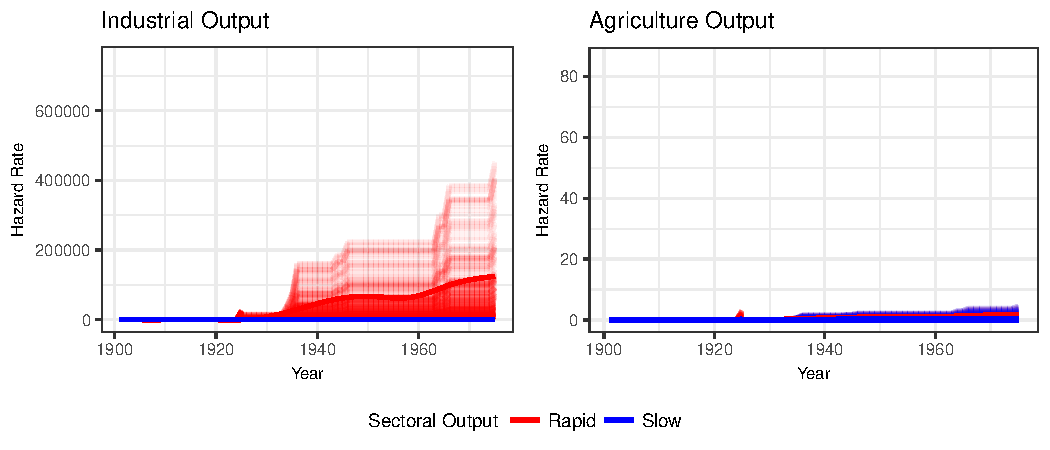
\includegraphics[scale=0.4]{/Users/hectorbahamonde/Dissertation/Papers/Earthquake_Paper/figure/simulation:plots-1.pdf}
	\end{figure}
\end{columns}
\end{frame}

\subsection{Published papers: Additional slides}

\miniframesoff
\begin{frame}\frametitle{\hypertarget{mart_paper}{{\scriptsize{``{\input{/Users/hectorbahamonde/research/Inequality_State_Capacity/title.txt}\unskip}''}}{\tiny (EJPE, forthcoming)}}}

\begin{columns}

\column{0.5\textwidth}
{\color{ForestGreen}{State Capacity and Democracy Increase Inequality}}:
\begin{itemize}
	\item We used a novel measurement of state capacity (cumulative census administration)
	\item {\bf Data and methods}: 126 countries (1970-2013), and FE panel regressions.
\end{itemize}

\column{0.5\textwidth}
	\begin{figure}[H]
		\vspace{0.5cm}
		\hspace{-1.3cm}
		\includegraphics[scale=0.12]{/Users/hectorbahamonde/research/Inequality_State_Capacity/Cum_Census_Map.jpeg}
	\end{figure}
\end{columns}
\end{frame}

\miniframesoff
\begin{frame}\frametitle{\hypertarget{mart_paper}{{\scriptsize{``{\input{/Users/hectorbahamonde/research/Inequality_State_Capacity/title.txt}\unskip}''}}{\tiny (EJPE, forthcoming)}}}

\begin{columns}

\column{0.5\textwidth}
{\color{ForestGreen}{State Capacity and Democracy Increase Inequality}}:
\begin{itemize}
	\item We find that democracy combined with state capacity increases inequality overtime.
	\item Relationship operates through the effect of high-capacity states and democracy on FDIs.
\end{itemize}

\column{0.5\textwidth}
	\begin{figure}[H]
		\vspace{-1cm}
		\hspace{-1.3cm}
		\includegraphics[scale=0.2]{/Users/hectorbahamonde/research/Inequality_State_Capacity/int_effect.png}\caption*{\scriptsize{{\color{ForestGreen}Marginal Effect (interaction effect): Inequality Increases.}}}
	\end{figure}
\end{columns}
\end{frame}


\miniframesoff
\begin{frame}[fragile]\frametitle{\hypertarget{vote_selling_paper}{{\scriptsize{``{\input{/Users/hectorbahamonde/research/Vote_Selling/title.txt}\unskip}''} {\tiny(AP, forthcoming)}}}}

\begin{columns}

\column{0.5\textwidth}
{\color{ForestGreen}{Original Survey Experiment}}:
\begin{itemize}
	\item {\bf Data and methods}: List experiment well suited to study behaviors subject to social desirability bias (such as selling one's vote) .
	\item N=1,479.
\end{itemize}

\column{0.5\textwidth}
    \begin{lstlisting}[language=tex, basicstyle=\tiny, frame=lrtb, numbers=none, style=base]
Now, you will have to type HOW MANY, if any, of the following illegal activities you might engage in, assuming you would not go to jail.

(1) steal an iPod from a large department store
(2) speed on the highway because you are late for work/school
(3) download your favorite music from the internet illegally

Type in HOW MANY (NOT WHICH), if any, of these things you would do.
\end{lstlisting}
\end{columns}
\end{frame}




\miniframesoff
\begin{frame}[fragile]\frametitle{\hypertarget{vote_selling_paper}{{\scriptsize{``{\input{/Users/hectorbahamonde/research/Vote_Selling/title.txt}\unskip}''} {\tiny(AP, forthcoming)}}}}

\begin{columns}

\column{0.5\textwidth}
{\color{ForestGreen}{Original Survey Experiment}}:
\begin{itemize}
	\item {\bf Data and methods}: List experiment well suited to study behaviors subject to social desirability bias ({\color{red}such as selling one's vote}) .
	\item N=1,479.
\end{itemize}

\column{0.5\textwidth}
    \begin{lstlisting}[language=tex, basicstyle=\tiny, frame=lrtb, numbers=none, style=base]
Now, you will have to type HOW MANY, if any, of the following illegal activities you might engage in, assuming you would not go to jail.

(1) steal an iPod from a large department store
(2) speed on the highway because you are late for work/school
@(3) sell your vote to a candidate for $100@
(4) download your favorite music from the internet illegally

Type in HOW MANY (NOT WHICH), if any, of these things you would do.
\end{lstlisting}
\end{columns}
\end{frame}


\miniframesoff
\begin{frame}\frametitle{\hypertarget{vote_selling_paper}{{\scriptsize{``{\input{/Users/hectorbahamonde/research/Vote_Selling/title.txt}\unskip}''} {\tiny(AP, forthcoming)}}}}

\begin{columns}

\column{0.5\textwidth}
{\color{ForestGreen}{Original Survey Experiment}}:
\begin{itemize}
	\item 25\% of Americans are still willing to sell their vote (expensive). {\bf Data are representative at the country level!}
\end{itemize}

\column{0.5\textwidth}
	\begin{figure}[H]
		\vspace{-0.2cm}
		\hspace{-1.3cm}
		\includegraphics[scale=0.6]{/Users/hectorbahamonde/research/Vote_Selling/figure/list:analysis:social:desirability:plot-1.pdf}
	\end{figure}
\end{columns}
\end{frame}



\miniframesoff
\begin{frame}\frametitle{\hypertarget{brazil_paper}{{\scriptsize{``{\input{/Users/hectorbahamonde/research/Clientelism_paper/title.txt}\unskip}''} {\tiny(JPLA, 2018)}}}}

\begin{columns}

\column{0.7\textwidth}
{\color{ForestGreen}{Matching methods for observational data, clientelism and inequality in Brazil}}:
\begin{itemize}
	\item Challenges the idea that only the poor are always targeted for clientelism.
		\begin{enumerate}
			\item Wealthy individuals living in neighborhoods with lots of poor people are targeted too (Q1): {\bf they are more noticeable (i.e., accountable)!}
			\item Poor individuals living in neighborhoods with lots of poor people are targeted too only in context of high contestation (Q4).
		\end{enumerate}
\end{itemize}

\column{0.4\textwidth}
	\begin{figure}[H]
		\vspace{-0.2cm}
		\hspace{-0.5cm}
		\includegraphics[scale=0.45]{/Users/hectorbahamonde/research/Clientelism_paper/figure/plot:four:quadrants-1.pdf}
	\end{figure}
\end{columns}
\end{frame}



\miniframesoff
\begin{frame}\frametitle{\hypertarget{translog_paper}{{\scriptsize{``Employment Effects of Covid-19 across Chilean Regions: An Application of the Translog Cost Function''} {\tiny(Regional Science Policy and Practice, 2020)}}}}

\begin{columns}

\column{0.7\textwidth}
{\color{ForestGreen}{Regional effects of Covid Pandemic}}:
\begin{itemize}
	\item Aggregated translog cost function (2013–2018) we provide forecasts of regional employment loses (between 700K-800K). 
	\item Relative impacts were spatially heterogeneous.
\end{itemize}

\column{0.4\textwidth}
	\begin{figure}[H]
		\vspace{-1cm}
		\hspace{-0.5cm}
		\includegraphics[scale=0.15]{/Users/hectorbahamonde/research/COVID/map.png}
	\end{figure}
\end{columns}
\end{frame}


\end{document}

